\section{Methods}
\numberwithin{equation}{section}
This section explains methods used to reduce runtime and
increase precision.

\subsection{Simulation data}
All plots and graphics of this sections
are based on simulations of the same gain medium (similar to Figure \ref{graphic:samples_reduced})
with the following properties:
\\
\\
\begin{tabular}{| l | l |}
\hline
Points per plane        & 321\\
\hline
Sample points           & 3210\\
\hline
Planes                  & 10\\
\hline
Triangles               & 600\\
\hline
Prisms                  & 5400\\
\hline
Height                  & 0.6 cm\\
\hline
Surface area            & 4 x 4 cm\\
\hline
Material                & YAG crystal\\
\hline
Spectrum                & Monochromatic\\
\hline
\end{tabular}

\subsection{Parallel methods}
\label{subsec:parallel_methods}
Moving from a single CPU to a multiple
GPU implementation is not so much about changing the overall algorithm,
but more about efficient utilisation of the GPU ressources. 
By using CUDA\cite{cuda} as a parallel computing platform created by NVIDIA\cite{nvidia},
it is possible to obtain high performance with a high level 
programming model (similar to C). Therefore the parallelization was pushed on CUDA-thread, 
CUDA-block and multiple GPU level to reach a good speedup compared to 
the sequential implementation.
In the following, the used parallelization
techniques and their implementations are explained.

\subsubsection{Rays as GPU threads}
    The Raytracing of every ray can be done independently through the mesh
    structure.  Exploiting this parallelism provides a great opportunity to
    boost performance. Figure \ref{graphic:kernel} demonstrates the distribution
    of rays. For each sample point $s_i$, a kernel consisting of a grid of 200
    CUDA blocks is spawned. Each of those blocks contains 128 CUDA threads.
    The maximum amount of used thread blocks is bounded to the used
    mersenne twister implementation\cite{mersenne_twister} as random number generator.
    The number of threads per block was determined by the CUDA Occupancy 
    Calculator\cite{occupancy_calculator} with the object to obtain the
    maximum occupancy.
    
    Since there are $N$ rays to calculate for each sample point, each thread
    traces up to $t = \lceil\frac {N}{200\cdot128}\rceil$ rays and computes the
    corresponding gain values using the following cycle (see Figure
    \ref{graphic:algorithm_steps}):
    
    \begin{enumerate}
      \item Get current sample point $s_i$
      \item Request a prism $x$ to start ray from
      \item Generate start point $r_{i,u}$ inside this prism 
      \item Generate ray $\overrightarrow{r_{i,u}s_i}$
      \item Calculate the partial gains for $\overrightarrow{r_{i,u}s_i}$:
        \begin{enumerate}
          \item find intersection between $\overrightarrow{r_{i,u}s_i}$
            and $x$\label{goto:5a}
          \item calculate length $l_x$ of partial ray $\overrightarrow{r_{i,u}r_x}$
          \item calculate $partial\_gain(x)$ \eqref{eq:partial_gain}
          \item if the ray did not reach $s_i$, determine neigboring prism $x'$,
            set $x := x'$ and $r_x$ as the new start point. goto \ref{goto:5a} 
        \end{enumerate}
      \item Calculate $gain(\overrightarrow{r_{i,u}s_i})$ \eqref{eq:gain}
      \item Add gain to gain of the other rays in the thread
    \end{enumerate}
    After a maximum of $t$ iterations, the thread has computed its share and
    adds its accumulated gain atomically to the results of the other threads
    \eqref{eq:monte_carlo_ase}.

\begin{figure}[H]
  \centerline
  {\resizebox{0.5\textwidth}{!}{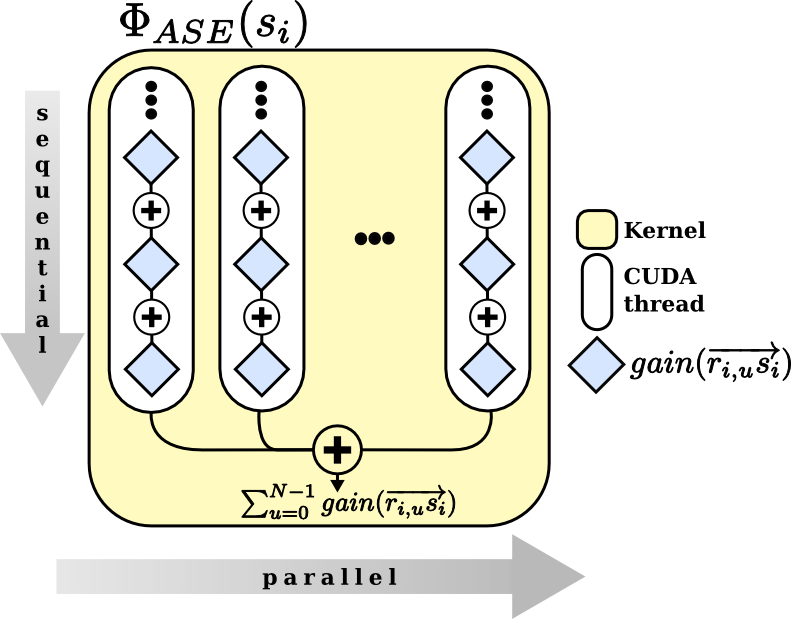
\includegraphics{graphics/kernel_detail3.png}}}
  \caption{$\Phi_{ASE}$ kernel with CUDA threads}
  \label{graphic:kernel}
\end{figure}

\begin{figure}[H]
  \centerline
  {\resizebox{0.45\textwidth}{!}{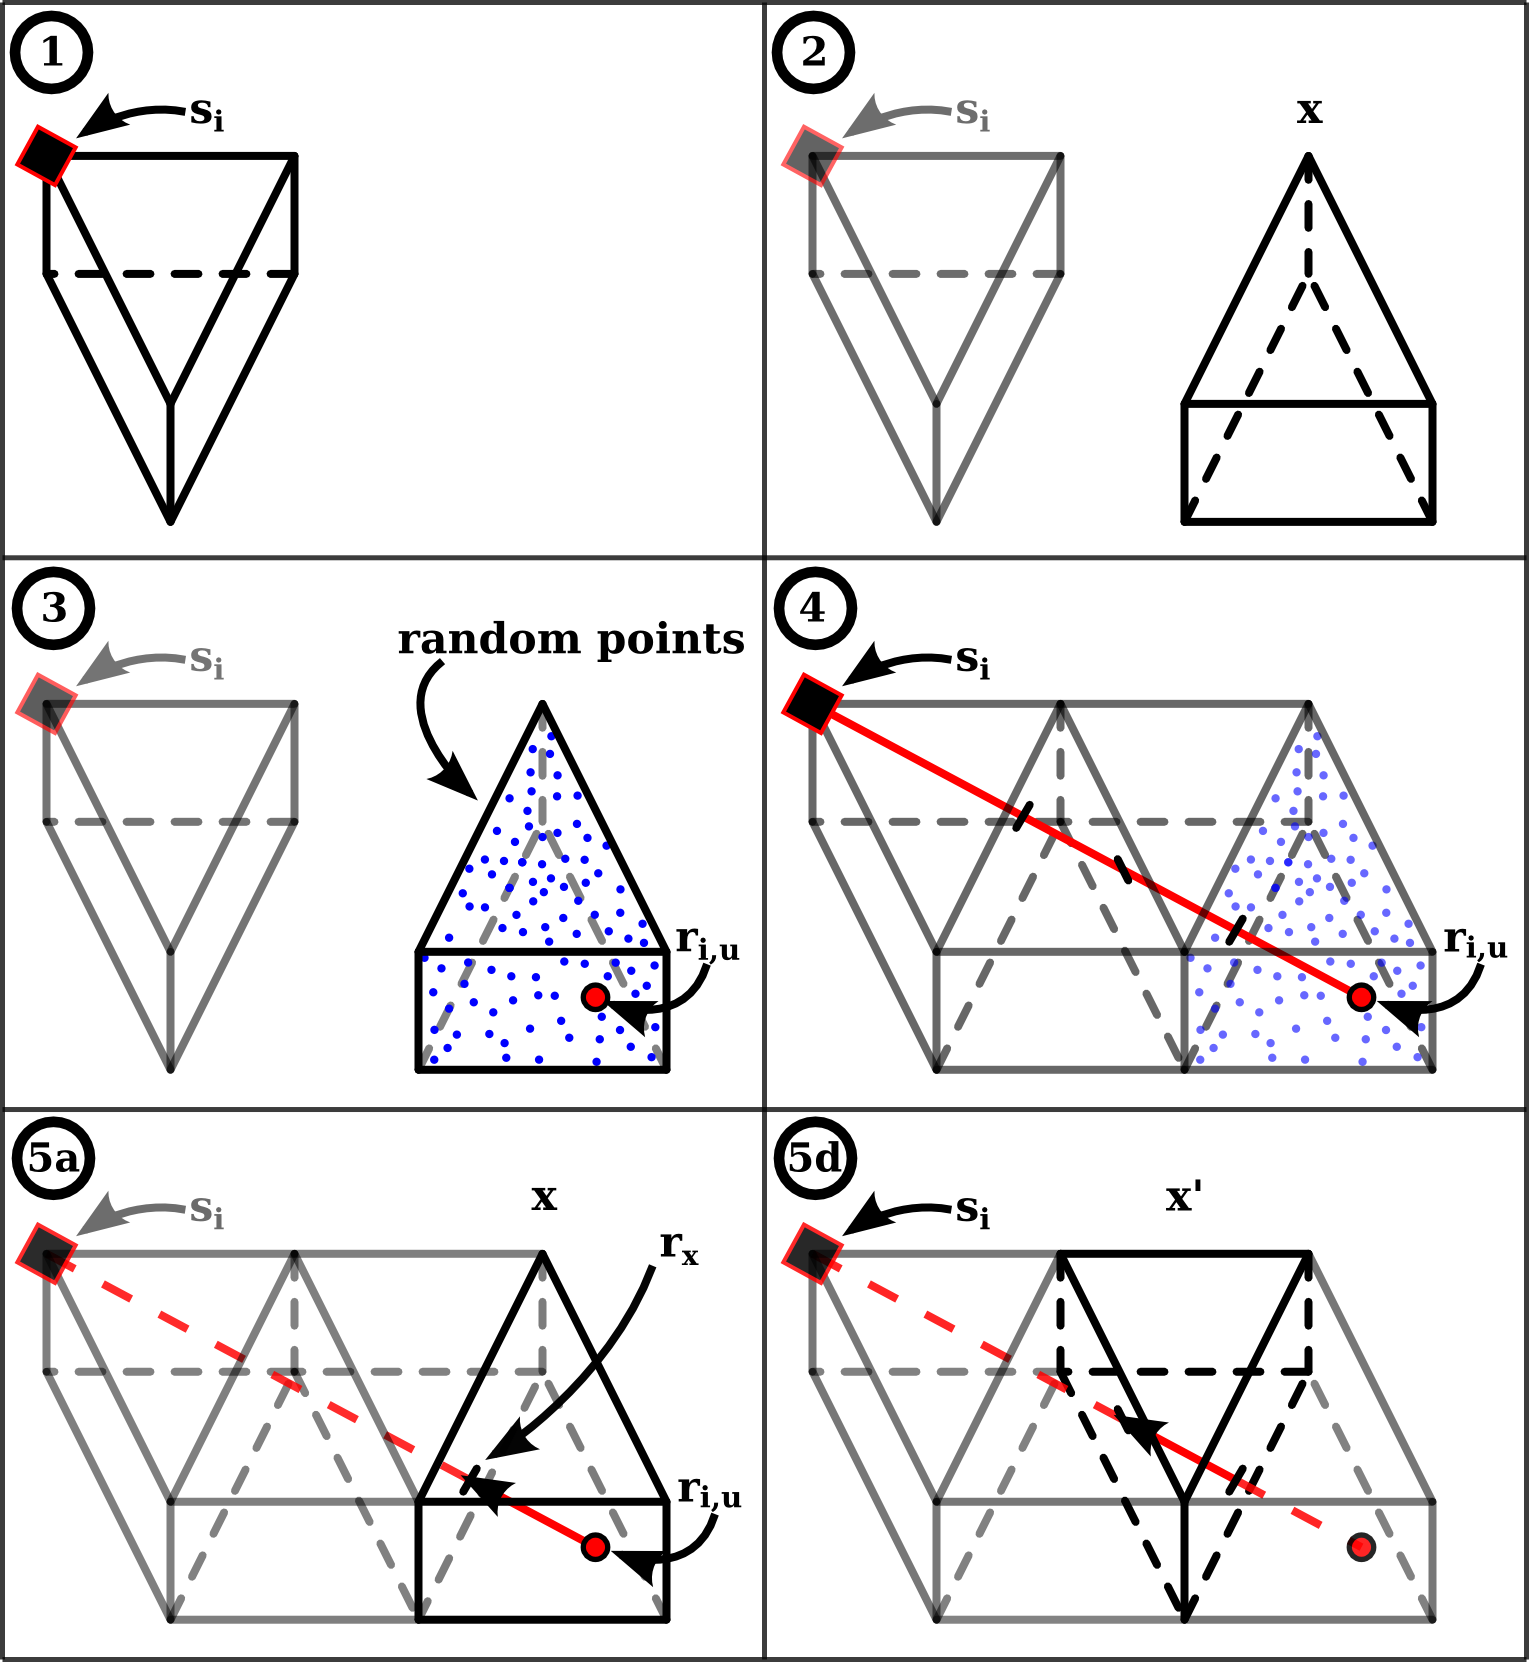
\includegraphics{graphics/iteration_detail4.png}}}
  \caption{steps for a single ray within a CUDA thread}
  \label{graphic:algorithm_steps}
\end{figure}

Furthermore, successive threads start rays from a similar origin, which results
in similar paths through the mesh structure and therefore similar prisms. This
leads to better utilisation of the GPU L1 cache and higher performance.

Since each distinct ray potentially has a different path through the gain
medium, the execution times between threads will differ substantially. In case
of a static mapping from threads to rays (i.e. strided access), one thread can
end up calculating many rays with long paths. If there are still many of those
rays remaining, the thread has to continue working for a long time, while all
other threads are already finished. These idle threads are unable to
participate, leaving many resources on the device unused.

To improve load balancing between the threads, each thread block fetches a
workload equal to its size and executes it completely before determining a new
workload. Therefore, if a single thread calculates a ray with a very long path,
only threads in the same block depend on the duration of one long ray.
Meanwhile, threads in other blocks can pick up more work. Thus, most resources
can contribute to the computation.
    
%\begin{figure}[H]
%  \centerline
%  {\resizebox{0.35\textwidth}{!}{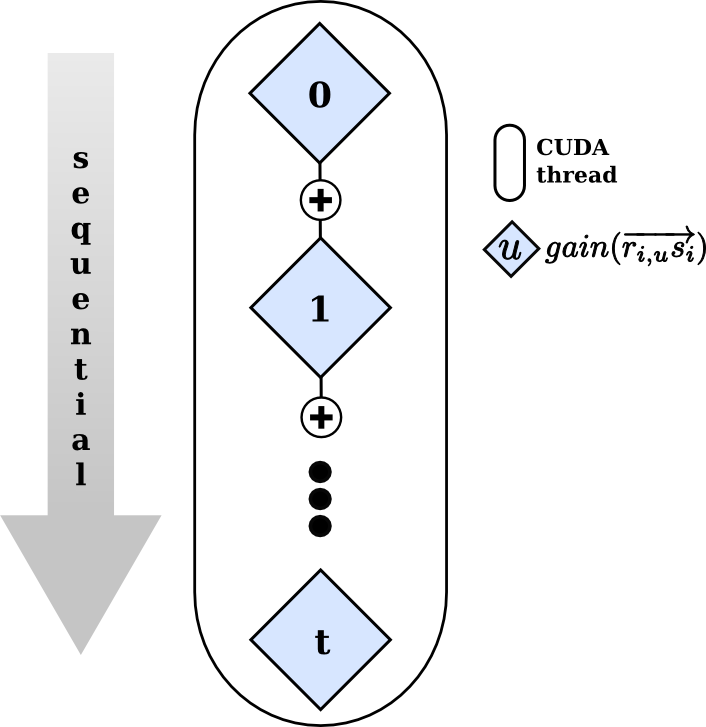
\includegraphics{graphics/thread_detail1.png}}}
%  \caption{Multiple gain calculations within a single CUDA thread}
%  \label{graphic:thread_detail}
%\end{figure}

\subsubsection{Sample Points on multiple GPUs}
\label{subsubsec:multigpu}

Each Monte Carlo experiment (see section \ref{eq:monte_carlo_ase}), calculates
the $\Phi_{ASE}(s_i)$ value of a sample point $s_i$ independently from each
other. Thus, every $\Phi_{ASE}(s_i)$ calculation can be executed as a
self-contained CUDA kernel and therefore sample points can be distributed to
several devices.

Consider a MPI environment with $k$ nodes, each hosting 1 GPU. Furthermore, one
node is used as a headnode responsible for distributing the workload. The
headnode holds a queue of all sample points. Each node requests a new sample
point and begins the calculation. As soon as the calculation is finished, a node
is able to request new work indepently from the other nodes (Figure
\ref{graphic:multigpu}). This form of load balancing is especially important in a
scenario with varying workloads for each sample point (see section
\ref{subsec:adaptive_sampling}).

As a result, the speedup is almost linear in the number of GPUs. This was
verified with up to 64 nodes.
    
\begin{figure}[H]
  \centerline
  {\resizebox{0.45\textwidth}{!}{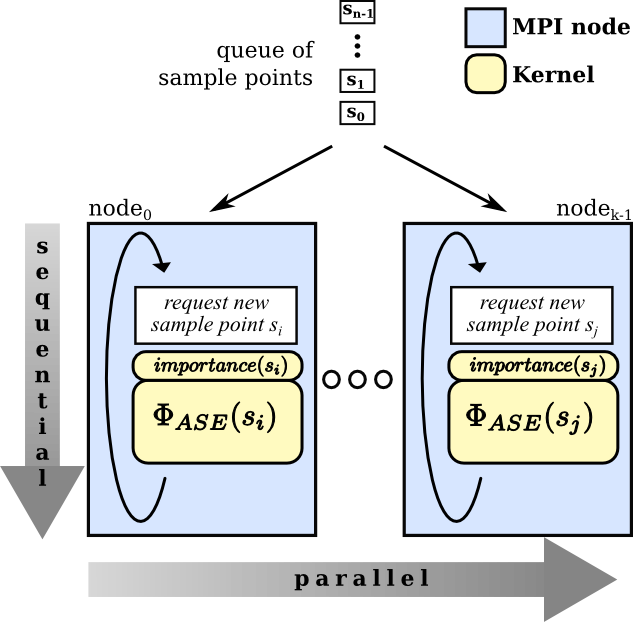
\includegraphics{graphics/multigpu_partitioning3.png}}}
  \caption{partitioning of the workload to multiple devices}
  \label{graphic:multigpu}
\end{figure}

\subsection{Importance sampling (IS)}
\label{subsec:importance_sampling}
Importance sampling is a well known technique in the domain
of statistics \cite{importanceSamplingSource}. It has to be calculated 
before every  $\Phi_{ASE}$ kernel (see Figure \ref{graphic:multigpu}) and is used 
to figure out which areas are most important to the result.

The objective is to distribute N rays to P prims of the active gain medium.
This is done by introducing a center point $c_x$ and triangle surfaces $T_x$ for every prism $x$ with $x \in \{0,...,P\}$.
 The rays per prism $rays_x$ and importance $imp_x$ for sample point $s_i$ are calculated as follows:
\begin{align}
  rays_x       &= \left\lfloor\frac{gain(\overrightarrow{c_xs_i}) \cdot N}{\sum^{P}_{j=0} gain(\overrightarrow{c_js_i})}\right\rfloor\\
imp_x &= 
\begin{cases}
\frac{T_x}{T_{total}} \cdot \frac{N}{rays_x} &rays_x > 0\\
0 &\text{otherwise}
\end{cases}
\end{align}

Using importance sampling leads to the modified gain calculation:
\begin{align}
  gain\_imp(\overrightarrow{r_{i,u,x}s_i})        &= gain(\overrightarrow{r_{i,u}s_i}) \cdot imp_x
\end{align}


The result of the importance sampling is a schedule for $s_i$, that
describes in which prism each ray starts.
This method has a strong impact on the precision of the simulation
and is able to reduce strong peaks in Monte Carlo simulations.

To show the impact of importance sampling in $\Phi_{ASE}(s_i)$, the difference
\[\Phi_{ASE\Delta} = |\Phi_{ASE~IS}(M) - \Phi_{ASE~Uniform}(N)|\] of the 
result with importance sampling ($IS$) and with uniform sampling ($Uniform$) was calculated with 
$N,M = 10^5$ rays per sample point (see Figure \ref{graphic:importance}). 
Then, N was increased in two steps by a factor of 10 for the simulation with uniform sampling.
The more rays are simulated, the smaller is $\Phi_{ASE\Delta}$, which 
means that the simulation
with importance sampling achieves the same results with less
rays per sample point. Thus, importance sampling can increase the
efficiency of Monte Carlo simulations by reducing variance 
and simulation runtime. 
\begin{figure}[H]
  \centerline
  {\resizebox{0.45\textwidth}{!}{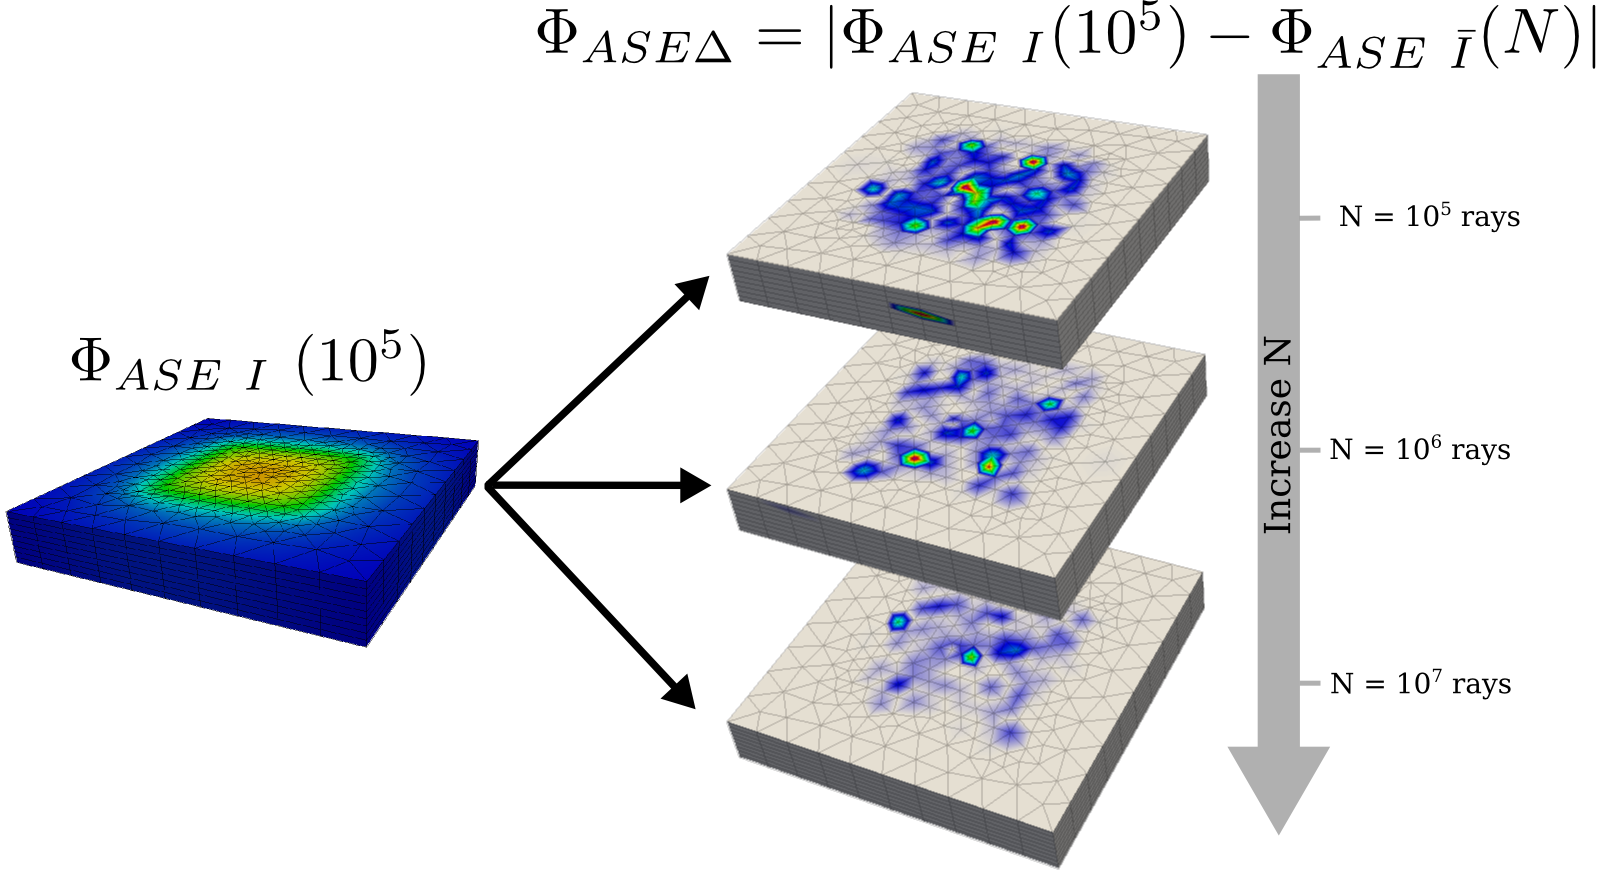
\includegraphics{graphics/phiASE_difference_new.png}}}
  \caption{$\Phi_{ASE\Delta}$ compared with increasing N}
  \label{graphic:importance}
\end{figure}

\subsection{Adaptive sampling (AS)}
\label{subsec:adaptive_sampling}
To assess the precision
and therefore the difference between the true and calculated value,
it is further determined the mean squared error (MSE):
\begin{align}
     f(\vec{s_i}) &= \frac{1}{N} \sum_{u=0}^{N-1} gain(\overrightarrow{r_{i,u}s_i})\\
     f^2(s_i)     &= \frac{1}{N} \sum_{u=0}^{N-1} gain(\overrightarrow{r_{i,u}s_i})^2\\
     MSE(s_i)     &= \sqrt{\frac{f^2(s_i) - f(s_i)^2}{N}}
\end{align}
Since most sample points $s_i$ have a low $MSE(s_i)$, there is no need
to sample them with a high number of rays. Only some outliers need to
be sampled with a higher resolution. This can be done with an adaptive
method, which allows to remove strong peaks in the result
of the simulation by either resampling these points with more rays.

Potential unbalanced load, because of variable number of rays per sample 
in a multi GPU scenario, is reduced by the MPI load balancer (see section
\ref{subsubsec:multigpu}).

For comparision, the impact of importance sampling
on the MSE values is shown (see Figure~\ref{plot:importance2}). 
Importance sampling alone already reduces the MSE values for
many sample points considerable.
\begin{figure}[H]
  \centerline{
    \resizebox{0.5\textwidth}{!}{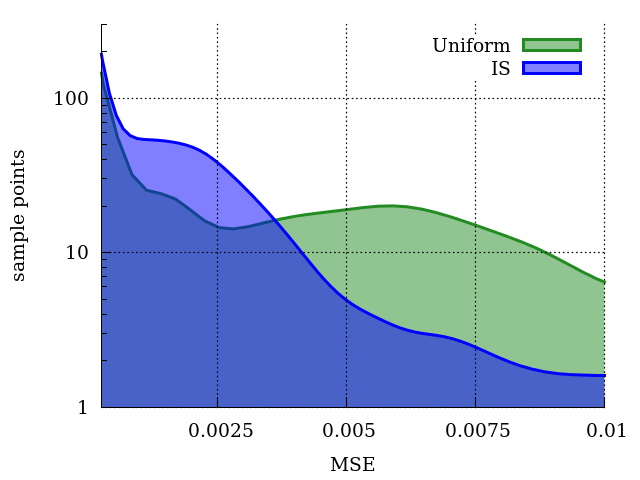
\includegraphics{plot/mse_importance.png}}}
  \caption{histogram of MSE values IS and Uniform sampling}
  \label{plot:importance2}
\end{figure}
By using also adaptive sampling, the MSE values are reduced to a specific MSE threshold.
Figure \ref{plot:adaptive} shows the histogramm of MSE values for a MSE threshold
of $0.005$. All sample points $s_i$ with $MSE(s_i) > 0.005$ were resampled with more rays
per sample point to lower their MSE value. The other sample points remained unchanged
to reduce calculation time.
\begin{figure}[H]
  \centerline{
    \resizebox{0.5\textwidth}{!}{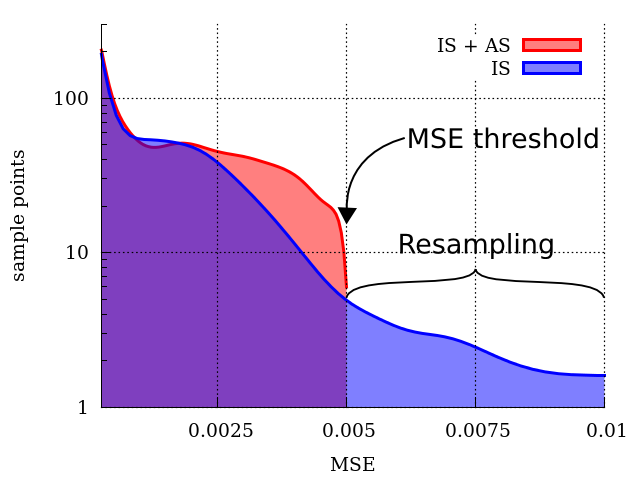
\includegraphics{graphics/mse_adaptive.png}}}
  \caption{histogram of MSE values IS and IS + AS}
  \label{plot:adaptive}
\end{figure}
The adaptive method will not reduce the average MSE over all sample points,
but it will reduce the maximal MSE values. Thus, using the adaptive
methods gives lower error by same calculation time.


\subsection{Repetitive sampling (RS)}
Repetitive sampling lowers the MSE values without increasing the number of rays by restarting the
simulation for a sample point with the same number of rays and a different random number 
generator. This can reduce the number of rays over all sample points and therefore
also runtime. Thus, repetitive sampling is an optimization over the adaptive sampling. 

Figure \ref{plot:repetitive} shows the sampling resolution
of the sample points in a histogram. Simulating with RS reduces
simulations sampled with $10^8$ rays by 319 sample points, resulting in 
$3\cdot10^{10}$ rays less to calculate. Because reducing the number of rays always
reduces runtime, it explains the difference in runtime
of 560s.
\begin{figure}[H]
  \centerline{
    \resizebox{0.5\textwidth}{!}{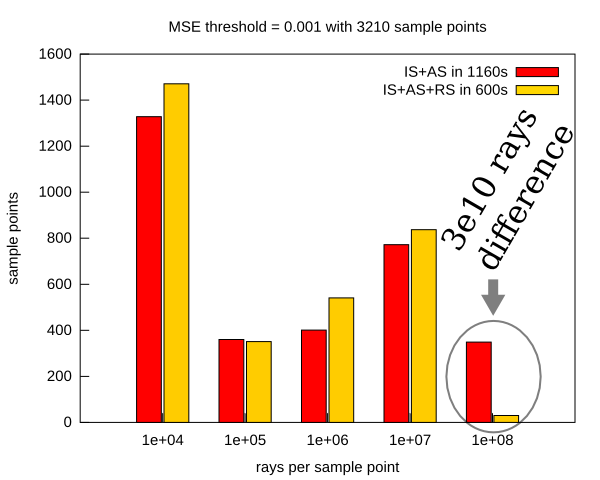
\includegraphics{graphics/repetitive_sampling.png}}}
  \caption{AS and RS compared by rays per sample point}
  \label{plot:repetitive}
\end{figure}

\subsection{Benefits of sample methods}
In this section, the presented methods IS, AS and RS are compared by duration
and precision.
In Figure \ref{graphic:methods_compare}, the runtime to reach an
MSE value of 0.01 was measured. It is evident that AS and RS perform
much better than Uniform or IS. 
\begin{figure}[H]
  \centerline{
    \resizebox{0.5\textwidth}{!}{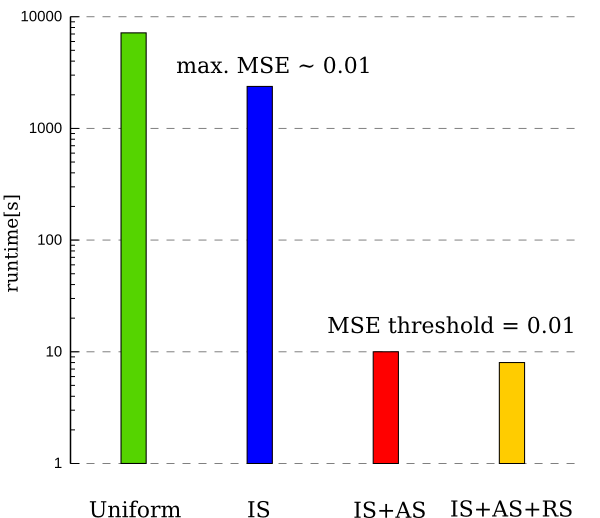
\includegraphics{graphics/methods_compare.png}}}
  \caption{Methods with same MSE value}
  \label{graphic:methods_compare}
\end{figure}
On the other hand, Figure \ref{graphic:methods_compare2} shows the MSE
distribution in the gain medium for a fixed runtime of 10s. Uniform and IS 
produce higher MSE values than AS or RS.
\begin{figure}[H]
  \centerline{
    \resizebox{0.5\textwidth}{!}{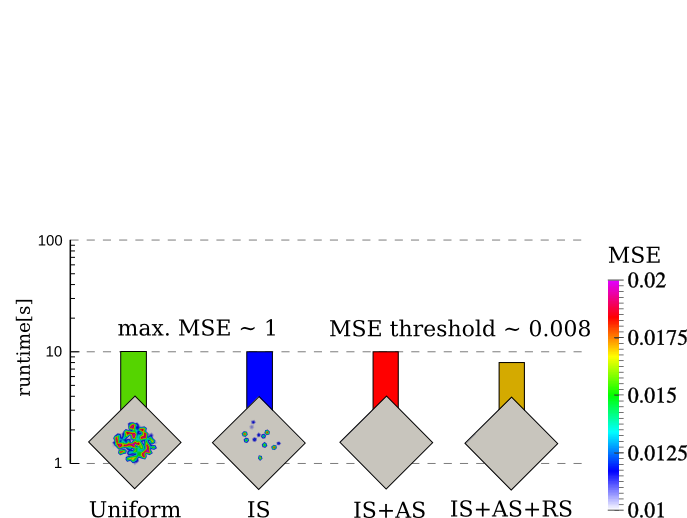
\includegraphics{graphics/methods_compare2.png}}}
  \caption{MSE distribution on gain medium for different methods}
  \label{graphic:methods_compare2}
\end{figure}
